\section{Grundlagen} % (fold)
\label{sec:grundlagen}

	\subsection{Temperaturmessung am Nullpunkt} % (fold)
	\label{sub:temperaturmessung_am_nullpunkt}

		Zur Messung sehr tiefer Temperaturen kann die Temperaturabhängigkeit des elektrischen Widerstandes ausgenutzt werden.
		Gute metallische Leiter wie Kupfer oder Platin zeigen einen in guter Näherung linearen Anstieg des Widerstandes mit der Temperatur.
		Bei wenigen Kelvin geht diese Linearität jedoch in einen abflachenden Restwiderstand über, der umso kleiner ist, je reiner das Metall.
		Die verschwindende Ableitung $\diff R/\diff T$ macht in diesen Bereich die Temperaturmessung also ungenau.
		Besser eignen sich hier Halbleiter wie beispielsweise Dioden.
		Hier werden die zum Stromfluss notwendigen freien Ladungsträger erst durch thermische Anregung erzeugt, weshalb der Widerstand bei tiefen Temperaturen stark ansteigt.
		Die Zusammenhänge sind in den Abbildungen \ref{diodenui} und \ref{pt1000} dargestellt:
		\begin{figure}[H]
			\center
			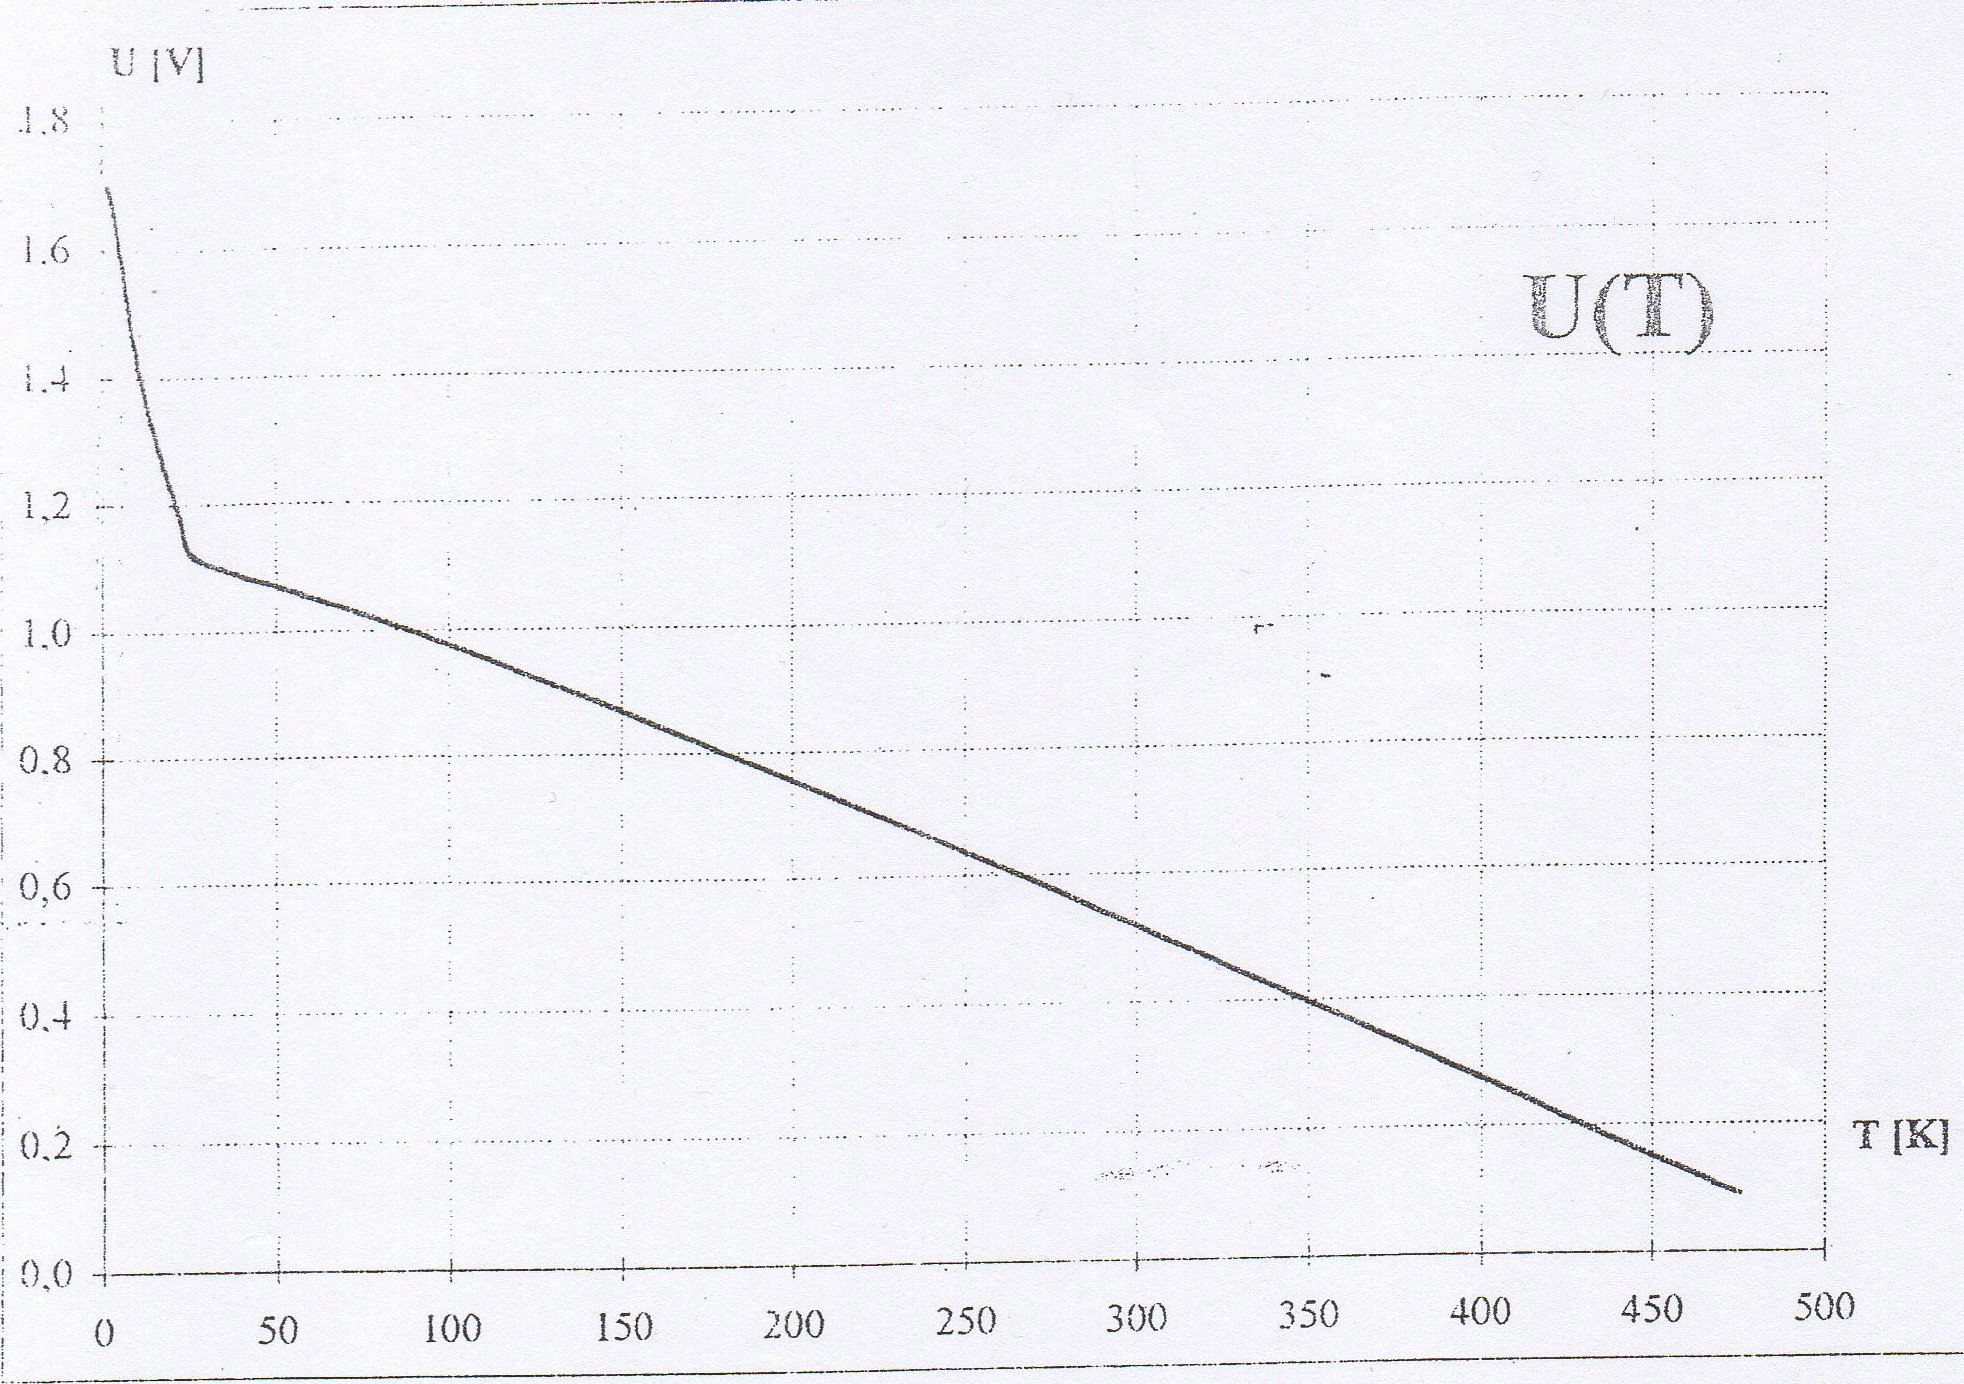
\includegraphics[scale=0.7]{messwerte/diodenui.jpg}
			\caption{$U$-$I$-Kennlinie einer Diode}
			\label{diodenui}
		\end{figure}
		\begin{figure}[H]
			\center
			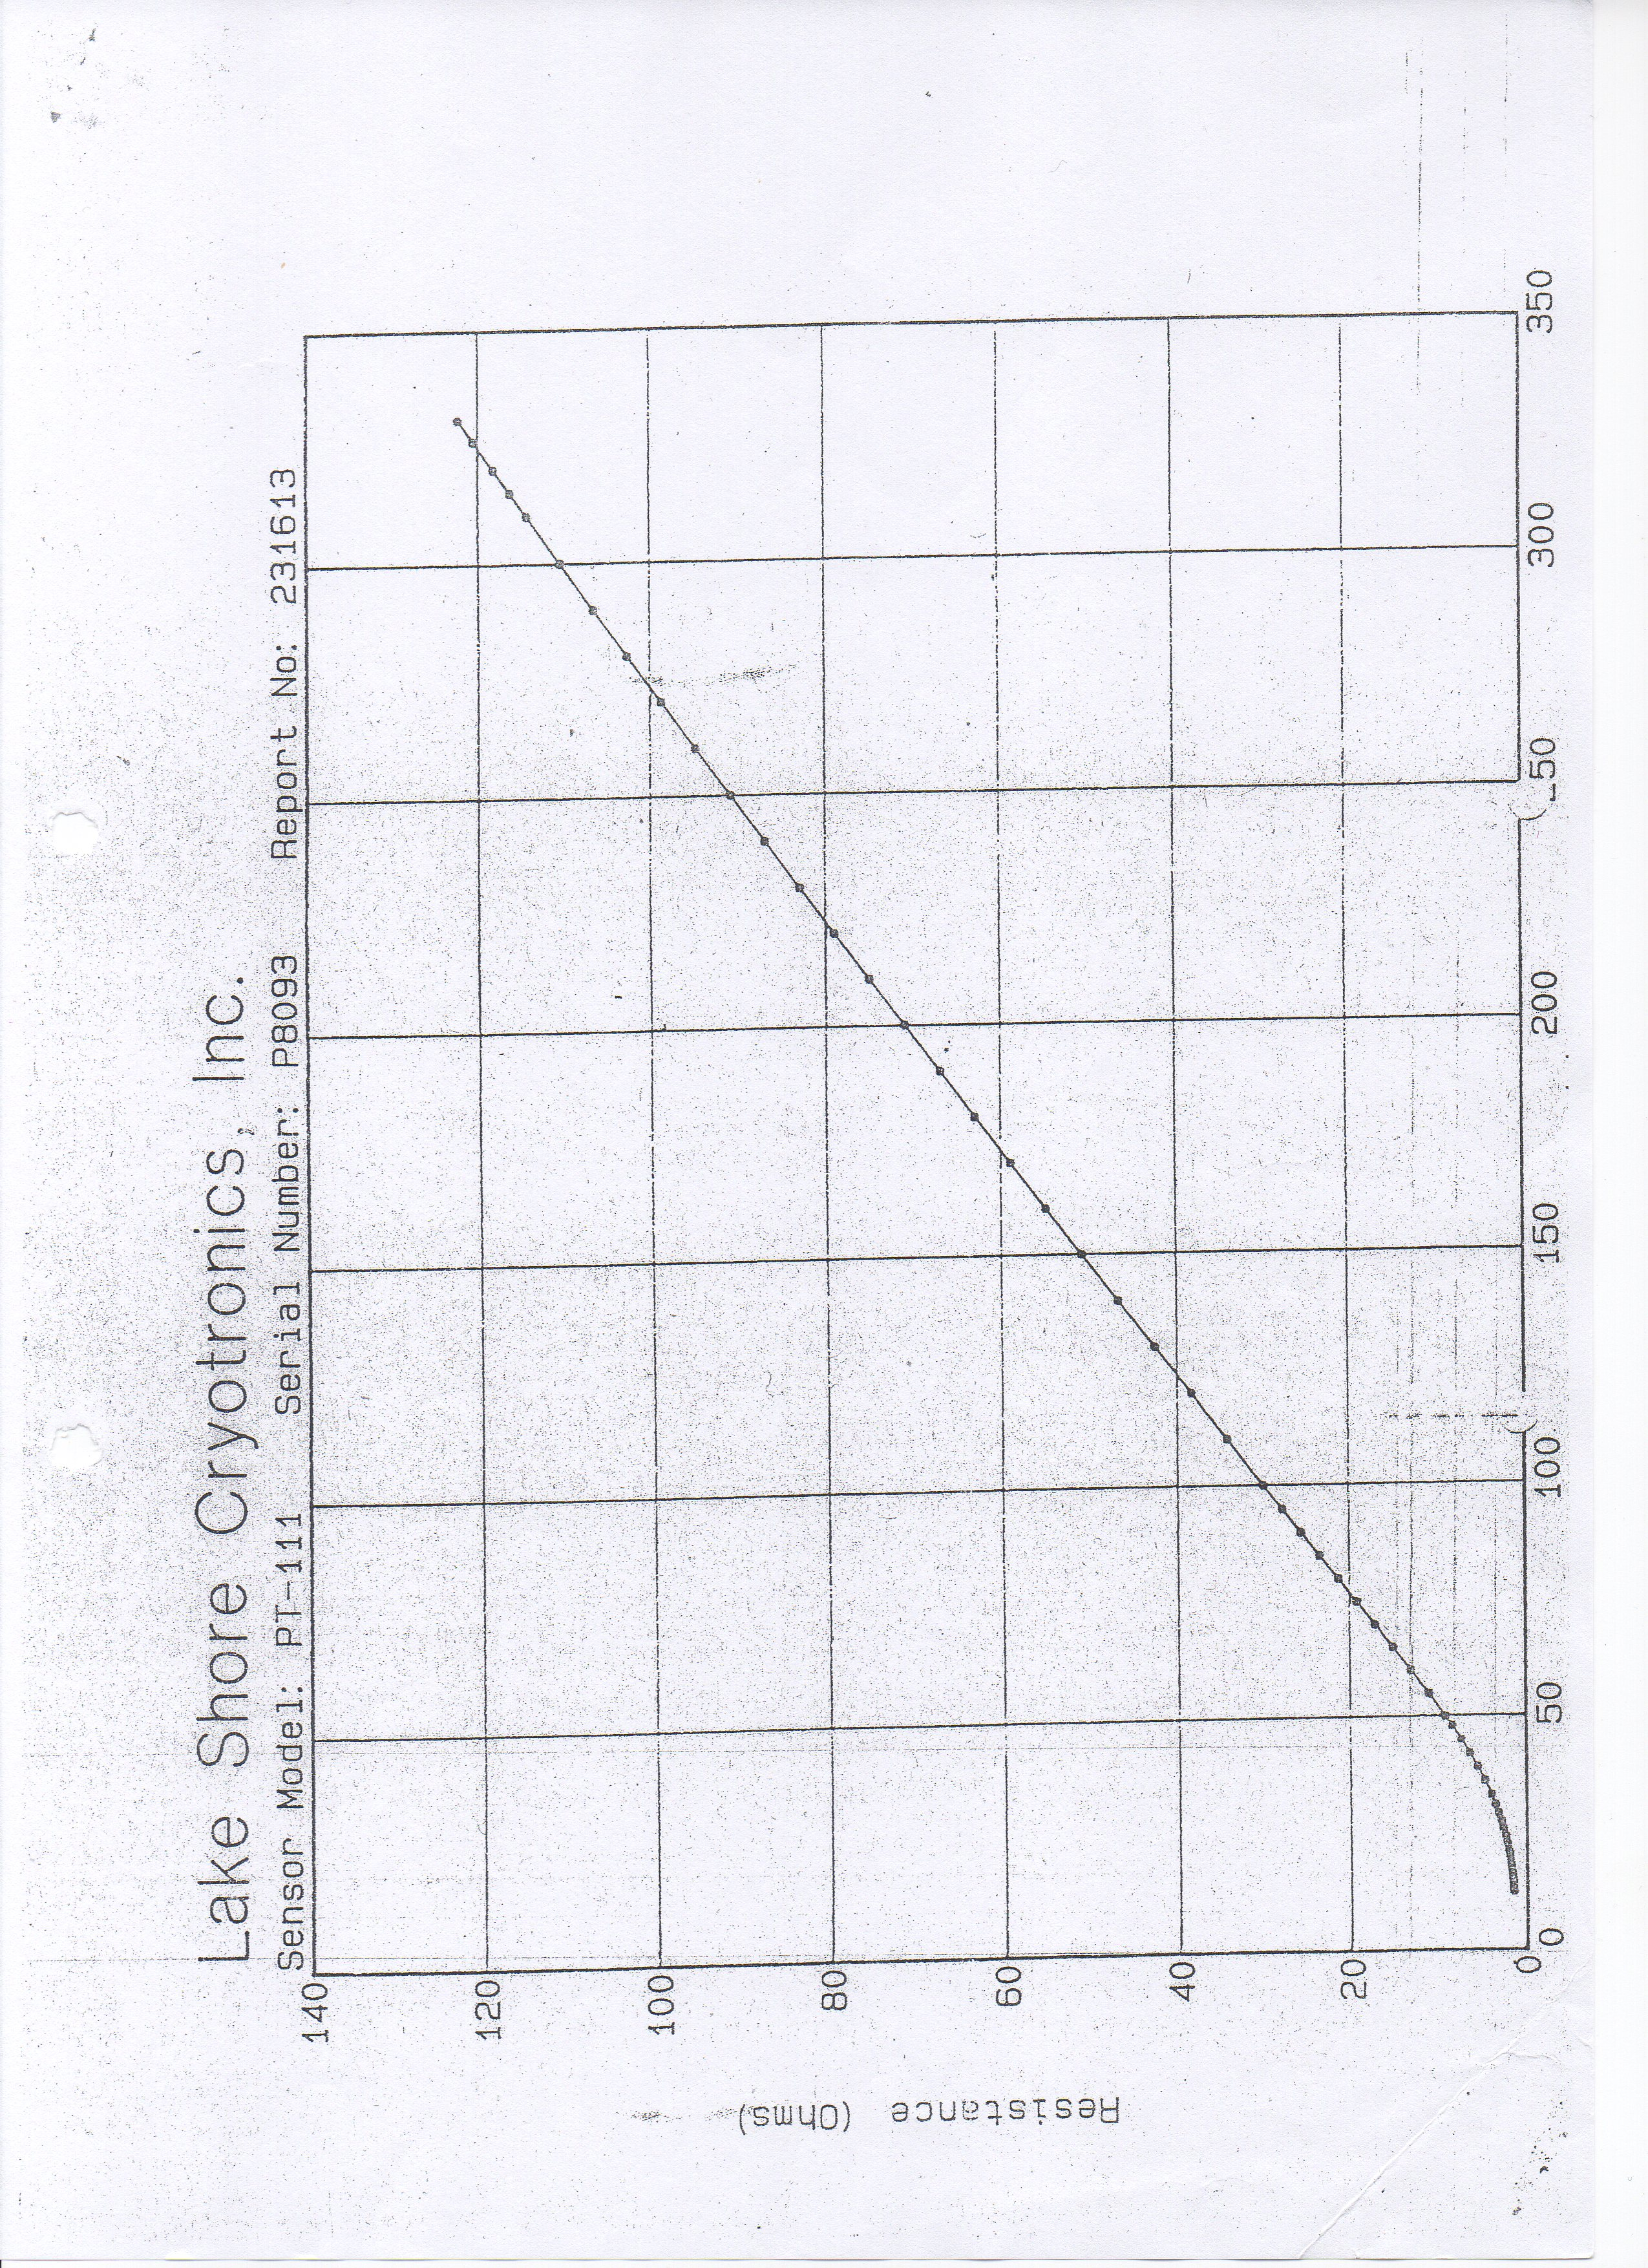
\includegraphics[scale=0.4, angle=-90]{messwerte/sl003.jpg}
			\caption{Kennlinie des Pt1000}
			\label{pt1000}
		\end{figure}
	
	% subsection temperaturmessung_am_nullpunkt (end)

	\subsection{Supraleitung und BCS-Theorie} % (fold)
	\label{sub:supraleitung_und_bcs_theorie}

		1913 untersuchte Kamerlingh-Ones das Verhalten des elektrischen Widerstandes von Quecksilber bei tiefen Temperaturen und fand heraus, dass der Widerstand bei $4.2\unit{K}$ sprunghaft um mehrere Größenordnungen viel. 
		Das Experiment hatte einen neuen Zustand der Materie aufgedeckt. 
		Heute lässt sich dieses Verhalten mit Hilfe der BCS-Theorie (nach ihren Begründern Bardeen, Cooper und Schrieffer) erklären.
		Sie erkannten, dass beim Übergang in den supraleitenden Zustand die Elektronen paarweise in einen Zustand kondensieren, in dem sie nach den Gesetzen der Quantenmechanik eine kohärente Materiewelle mit wohldefinierter Phase bilden.
		Die Elektronen wechselwirken hierbei über die Phononen, die Schwingungen des Kristallgitters.
		Je 2 Elektronen unterschiedlichen Spins bilden ein Cooper-Paar, wodurch sich der Gesamtspin demnach zu Null ergibt.
		Somit sind die Ladungsträger nicht länger Fermionen sondern Bosonen.
		Diese haben nun alle den gleichen Impuls und können nicht mehr mit dem Gitter wechselwirken, wodurch ein widerstandsloser Ladungstransport möglich wird.
	
	% subsection supraleitung_und_bcs_theorie (end)

	\subsection{Sprungtemperatur und kritischer Strom} % (fold)
	\label{sub:sprungtemperatur_und_kritischer_strom}
	
		Oberhalb einer bestimmten Temperatur zerbrechen die Cooper-Paare wieder in einzelne Elektronen und das ohmsche Verhalten setzt wieder ein.
		Die Sprungtemperaturen für verschiedene Metalle sind in Abbildung \ref{tallaalala} ersichtlich:
		\begin{figure}[H]
			\center
			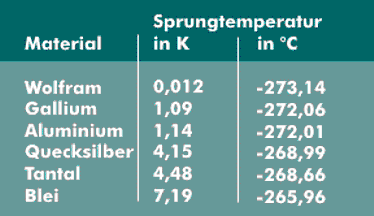
\includegraphics[scale=0.7]{messwerte/materialien-fuer-supraleiter-und-deren-sprungtemperaturen-in-kelvin-und-grad-celsius.png}
			\caption{Tabelle der Sprungtemperaturen verschiedener Metalle \\(Quelle: www.itwissen.info)}
			\label{tallaalala}
		\end{figure}
		Supraleiter vom Typ I verdrängen alle äußeren Magnetfelder durch Oberflächenströme aus dem Inneren (auch Meißner-Ochsenfeld-Effekt).
		Ein von außen angelegtes Magnetfeld verringert somit die Sprungtemperatur zusätzlich, wobei sich der Zusammenhang annähernd quadratisch darstellt.
		Da auch fließende Ströme ein Magnetfeld verursachen ist die Sprungtemperatur auch von der Stromstärke im Supraleiter abhängig.
		Oberhalb eines bestimmten kritischen Stromes geht das Verhalten des Leiters ebenfalls wieder in den ohmschen Zustand über.

	% subsection sprungtemperatur_und_kritischer_strom (end)

	\subsection{Josephson-Kontakte} % (fold)
	\label{sub:josephson_kontakte}
	
		Ein Josephson-Kontakt kann mit Hilfe zweier Supraleiter, die durch eine dünne Isolierschicht (z.B. Oxidschicht) getrennt sind erzeugt werden.
		Bei einem angelegten Strom können nun Cooper-Paare durch die Oxid-Barriere tunneln und ermöglichen so ebenfalls einen verlustfreien Ladungstransport. 
		Genauer ist durch die unterschiedliche Phase der beiden Materiewellen in den Leitern schon ein Gleichstrom beim bloßen Berühren der Supraleiter möglich, welcher jedoch schwer zu messen ist.
		Bei einem angelegten Wechselstrom beobachtet man nun innerhalb eines kleinen Bereiches um $0\unit{A}$ das supraleitende Verhalten, oberhalb des kritischen Stromes (nur der Betrag ist entscheidend) fällt aber wieder Spannung über dem Kontakt ab.
		Bei angelegter Spannung hingegen ändert sich die Phase in den Leitern und somit auch ihre Differenz mit der Zeit. 
		Das Resultat ist ein hochfrequenter Wechselstrom, dessen Frequenz sehr rasch mit der Spannung zunimmt und über folgenden Zusammenhang beschrieben wird.
		\[ f = \dfrac{2eU}{h} \] \par
		Mit Hilfe eines Ringes aus zwei Supraleitern, die durch zwei gleiche Isolatoren getrennt sind, kann ein SQUID (\textbf{S}uperconducting \textbf{Q}uantum \textbf{I}nterference \textbf{D}evice) realisiert werden.
		Mit dessen Hilfe lassen sich sehr kleine Magnetfelder nachweisen.\\
		Die Funktionsweise eines SQUID basiert auf dem Effekt der Flussquantisierung in supraleitenden Ringen und dem Josephson-Effekt. 
		Aus quantenmechanischen Gründen kann durch einen supraleitenden Ring nur ein magnetischer Fluss fließen, dessen Größe ein ganzzahliges Vielfaches des magnetischen Flussquantums $\Phi_0 = 2.07\cdot 10^{-15}\unit{Vs}$ beträgt. 
		Ändert sich das äußere Magnetfeld, so wird im Ring ein elektrischer Kreisstrom angeregt, der gerade groß genug ist, um den magnetischen Fluss im supraleitenden Ring auf das nächstgelegene Vielfache des Flussquantums zu erhöhen oder zu verringern.
		Durch Messung der Strom- oder Spannungsänderung im Ring kann nun das durchströmende Magnetfeld sehr genau bestimmt werden.

	% subsection josephson_kontakte (end)

% section grundlagen (end)